%\documentclass[useAMS, usenatbib,usegraphicx,letter]{mn2e}
%\documentclass[11pt]{article}
\documentclass[reprint,aps,prd,superscriptaddress,showkeys,showpacs]{revtex4-1}
\usepackage{epsfig,amsmath,natbib}

\usepackage{aas_macros}
\usepackage{amssymb}
\usepackage{amsmath}
\usepackage{dsfont}
\usepackage{hyperref}
\usepackage{color}
\usepackage{pbox}
\usepackage{booktabs}
\usepackage{minted}

\hypersetup{
	colorlinks=false,
	citecolor=green
}
% \usepackage{graphicx}
% \usepackage{epstopdf}
% \usepackage{natbib}

%%%%%%%%%%%%%%%%%
%Custom commands%
%%%%%%%%%%%%%%%%%

\newcommand{\bb}[1]{\mathbf{#1}}
\newcommand{\bbh}[1]{\mathbf{\hat{#1}}}
\newcommand{\h}[1]{\hat{#1}}
\newcommand{\ttt}[1]{\texttt{#1}}
\newcommand{\LT}{\texttt{LensTools} }

%%%%%%%%%%%%%%%%%%%%%%%%%%%%%%%%%%%%%%%%%%%%%%

\begin{document}

\title{Mocking the Weak Lensing universe: the LensTools computing package}

\author{Andrea Petri}
\email{apetri@phys.columbia.edu}
\affiliation{Department of Physics, Columbia University, New York, NY 10027, USA}
\affiliation{Physics Department, Brookhaven National Laboratory, Upton, NY 11973, USA}

\date{\today}

\label{firstpage}

\begin{abstract}
We present a newly developed software package which implements a wide range of routines frequently used in Weak Gravitational Lensing (WL). With the continuously increasing size of the WL scientific community we feel that easy to use APIs for common calculations are a necessity to ensure efficiency and coordination across different working groups. Coupled with existing open source codes, such as \ttt{CAMB}\citep{CAMB} and \ttt{Gadget2}\citep{Gadget2}, \LT brings together a fully functional cosmic shear simulation pipeline which, complemented with a variety of WL feature measurement tools and parameter sampling routines, provides easy access to the numerics for theoretical studies of WL as well as for experiment forecasts. Being implemented in \ttt{python}\citep{python}, \LT takes full advantage of a range of state--of--the art techniques developed by the large and growing open--source software community \citep{scipy,pandas,astropy}.    
    
\end{abstract}


\keywords{Weak Gravitational Lensing --- Simulations}
\pacs{98.80.-k, 95.36.+x, 95.30.Sf, 98.62.Sb}

\maketitle


%%%%%%%%%%%%%%%%%%%%%%%%%% INTRO %%%%%%%%%%%%%%%%%%%%%%%%%%%%%%%%%%%%%%%%%%%%%%%%%%%%%%%%

\section{Introduction}
%
Cosmology is entering a new, data driven era. After the Cosmic Microwave Background (CMB) \citep{WMAP,PlanckXVI2013} provided strong experimental evidences of cosmological theories, a variety of different probes have been proposed to unveil the secret of the cosmos. Weak Gravitational Lensing uses the correlation between image distortions of background sources by Large Scale Structure (LSS) to infer cosmological parameters \citep{WLprimer}. Because WL probes are sensitive to the late universe, where the density fluctuations are in the non--linear regime, the cosmological information might not be all contained in quadratic features such as two--point correlation functions. In the theoretical study of more complicated WL features (see for example \citep{3pcf1,bispectrum1,moments1,peaks1} for a non comprehensive list), simulation pipelines play a vital role as in general these features cannot be predicted analytically from the cosmological parameters. In this work we present a flexible, customizable and easy to deploy WL simulation pipeline that bridges the gap between simulations of shear fields, feature measurement from simulated images and cosmological parameter estimation. The paper is organized as follows: first we give an overview of the shear field simulation routines and present the benchmarks for runtime and memory usage. We next outline the \LT image analysis capabilities as well as the parameter estimation routines. We then present a summary and discuss possible future developments. We complement our work with some illustrative coding examples that show how to operationally use use \LT for some of the former tasks.

%%%%%%%%%%%%%%%%%%% Shear simulations %%%%%%%%%%%%%%%%%%%%%%%%%%%%%%%%%%%%%%%

\section{Shear simulations} 

\subsection{Formalism}
%
In this paragraph we give an overview of the \LT shear field simulation pipeline. This is a series of routines that, broadly speaking, take a vector of cosmological parameters $\bb{p}$ and some resolution parameters to produce random realizations of shear fields $\pmb{\gamma}(\pmb{\theta})$ in that particular cosmology ($\pmb{\theta}=(\theta_x,\theta_y)$ is the angle on sky as seen from the observer). Given a background source at redshift $z_s$, the matter density fluctuations $\delta(\bb{x},z)$ in between the observer and the source will cause its apparent shape to be distorted; the cosmic shear $\pmb{\gamma}$ is a measurement of the apparent source ellipticity, assuming the unperturbed shape is a circle. The multi--lens--plane algorithm \citep{RayTracingHartlap} is a popular techique to compute light ray deflections across the path $z\in[z_s,0]$ and hence to compute the apparent source shape distortion. The mass distribution between the source and the observer is approximated as a sequence of two dimensional lenses perpendicular to the line of sight, of thickness $\Delta$ and a surface density $\sigma$ given by 

\begin{equation}
\label{surfacedensity}
\sigma(\bb{x},z) = \frac{3H_0^2\Omega_m\chi(z)}{2c^2a(z)}\int_\Delta dz'\delta(\bb{x},z')
\end{equation}
%
Where $\chi$ is the lens comoving distance and $a=1/(1+z)$ the scale factor. A light ray crossing a lens at redshift $z$ at a transverse position $\bb{x}$ will be deflected by a small angle $\pmb{\alpha}$ which can be shown to be the gradient of the 2D gravitational potential $\phi$ (see again \citep{RayTracingHartlap}) 
%
\begin{equation}
\label{poisson}
\begin{matrix}
& \nabla^2_\bb{x} \phi(\bb{x},z) = 2\sigma(\bb{x},z) \\ \\
& \pmb{\alpha}(\bb{x},z) = \nabla_\bb{x} \phi(\bb{x},z) \\ \\
& \bb{T}(\bb{x},z) = \nabla_\bb{x}\nabla_\bb{x}^T \phi(\bb{x},z)
\end{matrix}
\end{equation}
%
where we indicated $\bb{T}$ as the gradient of the deflection, which will be called \textit{shear tensor} throughout the rest of the paper. An example of a lens plane computed with the \LT pipeline according to equations (\ref{surfacedensity}),(\ref{poisson}) is shown in Figure \ref{lensplanefig}. 

\begin{figure*}
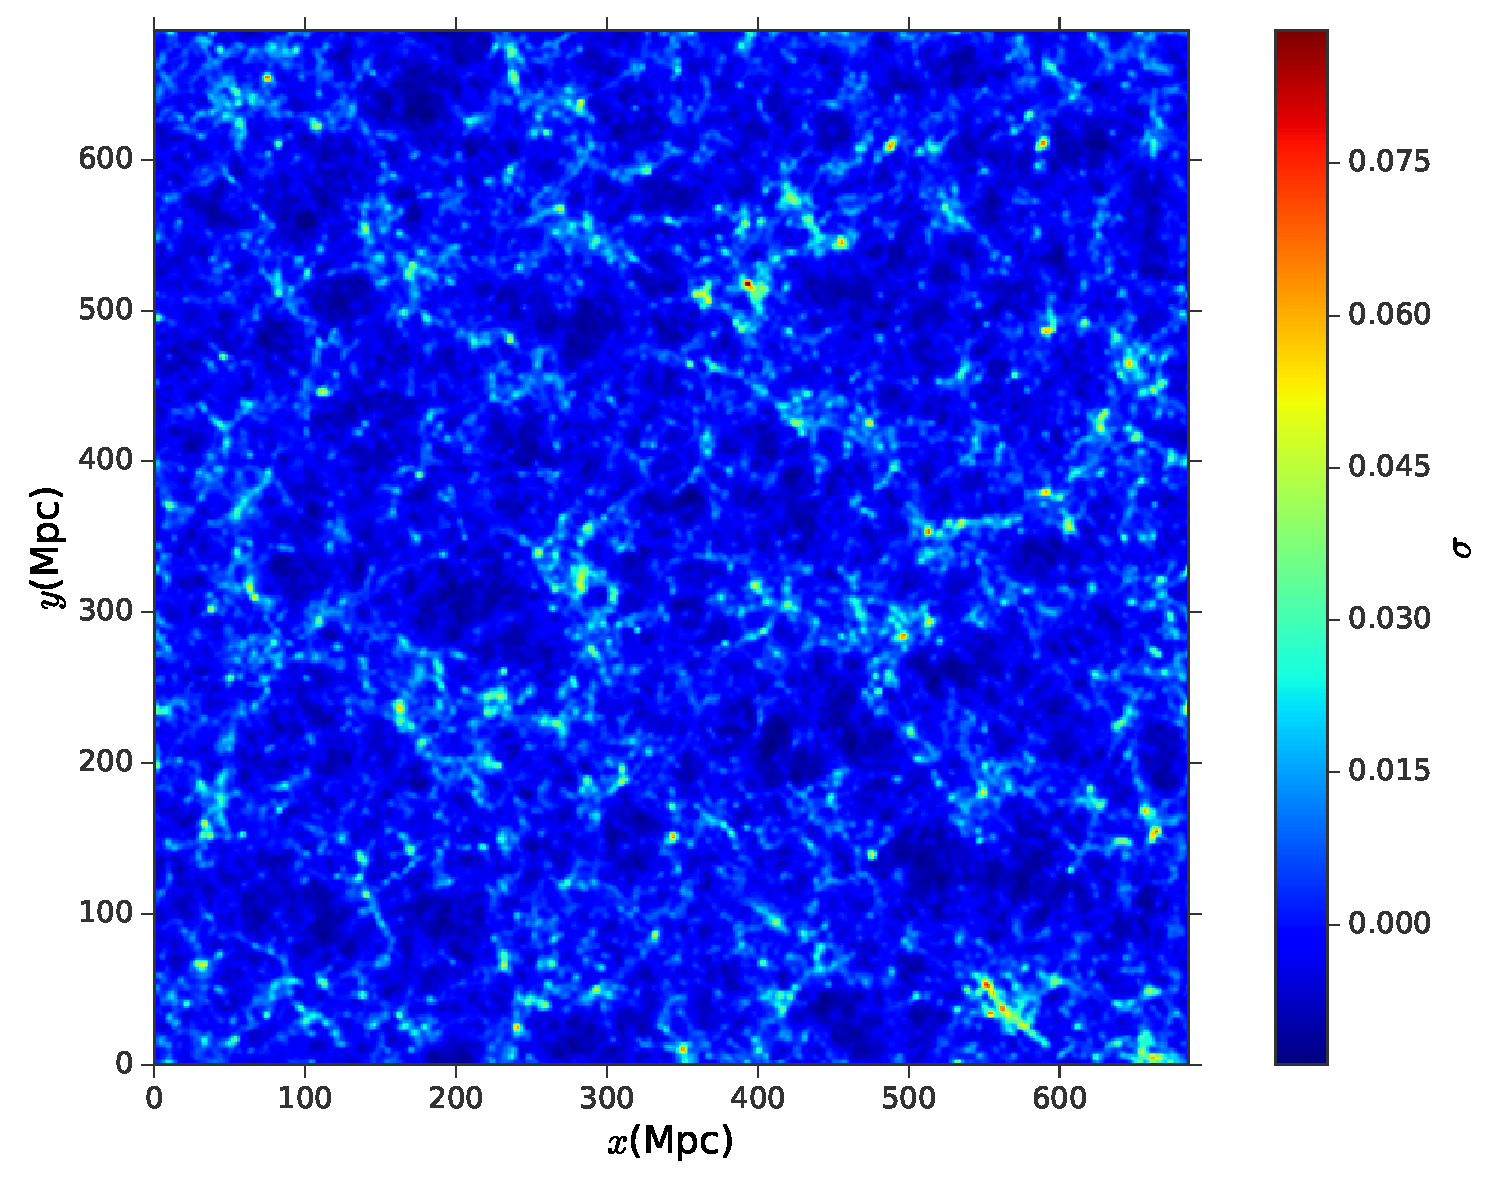
\includegraphics[scale=0.3]{Figures/lens_plane_density.eps}
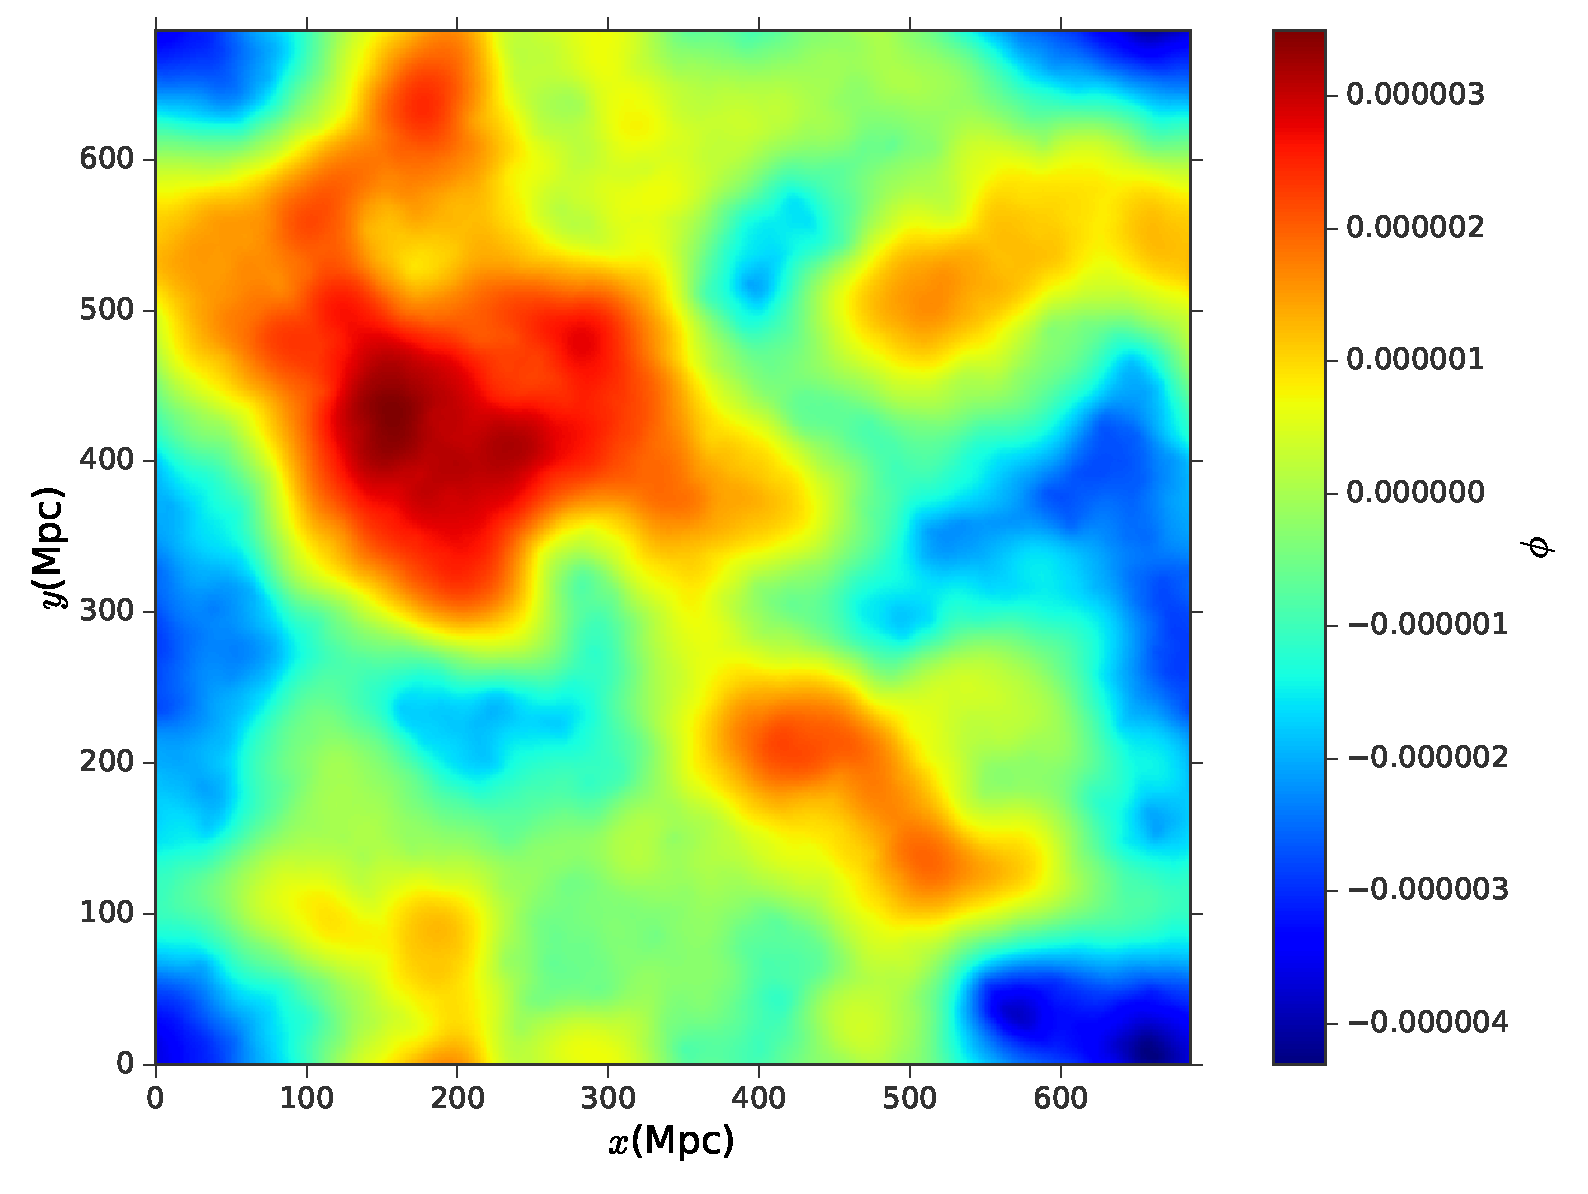
\includegraphics[scale=0.3]{Figures/lens_plane_potential.eps}
\caption{This figure shows a lens plane, computed with a gridding procedure based on equations (\ref{surfacedensity}),(\ref{poisson}). This lens plane has been generated from a $N$--body simulation of size $L_b=240\,{\rm Mpc}/h$ with $N_p=512^3$ particles at $z_s=2$. The plane resolution is $512\,$pixels per side. We show both the surface density $\sigma$ (left) and the lensing potential $\phi$ (right).}
\label{lensplanefig}
\end{figure*}
%
The trajectory of a light ray $\bb{x}(z)$ follows the geodesic equation

\begin{equation}
\label{geodesic3D}
\frac{d^2\bb{x}}{d\chi^2} = -\frac{2}{c^2}\nabla_\bb{x_\perp}\Phi(\bb{x},z)
\end{equation}
%
which can be translated into a second order differential equation for the light ray angular position $\pmb{\beta}(z)=\bb{x}_\perp(z)/\chi(z)$ as seen from the observer. Following \citep{RayTracingHartlap}, the trajectory of each light ray originating at $\pmb{\beta}(0)=\pmb{\theta}$ can be calculated solving numerically a discretized version of (\ref{geodesic3D}), assuming a finite number of lenses placed at a finite number of redshifts $\{z_k\}$:
%

\begin{widetext}

\begin{equation}
\label{geodesic2D}
\pmb{\beta}_{k} = \sum_{i=1}^k\delta\pmb{\beta}_i 
\end{equation}

\begin{equation}
\delta\pmb{\beta}_k = (A_k-1)\delta\pmb{\beta}_{k-1} + C_k\pmb{\alpha}_k 
\end{equation}

\begin{equation}
\bb{U}_{k} = \sum_{i=1}^k\delta\bb{U}_i 
\end{equation}

\begin{equation}
\delta\bb{U}_k = (A_k-1)\delta\bb{U}_{k-1} + C_k\bb{T}_k\bb{U}_k
\end{equation}

\end{widetext}
%
where $\bb{U}$ is the jacobian matrix of the trajectory $\pmb{\beta}$ with respect to the initial light ray position $\pmb{\theta}$, $\bb{U}_k=\nabla_{\pmb{\theta}}\pmb{\beta}_k(\pmb{\theta})$. The factors $A_k,C_k$ depend on the geometry of the lens system



\begin{equation}
A_k = \frac{\chi_{k+1}}{\chi_{k+2}}\left(1 + \frac{\chi_{k+2}-\chi_{k+1}}{\chi_{k+1}-\chi_k}\right) \,\,\,\, ; \,\,\,\, C_k = \frac{\chi_{k+1}}{\chi_{k+2}} - 1 \\ \\
\end{equation} 
%
where we use the subscript $k$ to indicate the redshift $z_k$ of the $k$--th lens for notational simplicity. After tracing the evolution of $\bb{U}$ from the observer to the source at $z_s$, we are able to evaluate the cosmic shear $\pmb{\gamma}$ and convergence $\kappa$ at $z_s$ looking at the components of $\bb{U}$
\begin{equation}
\bb{U}(\pmb{\theta},z_s) = (1-\kappa(\pmb{\theta}))\mathds{1}_{2\times2} - \gamma^1(\pmb{\theta})\sigma^3 - \gamma^2(\pmb{\theta})\sigma^1
\end{equation}
%
where we indicated $\mathds{1}_{2\times2}$ as the identity matrix and $\sigma^{1,3}$ as the first and third Pauli matrices. The iterative solution of (\ref{geodesic2D}) requires the knowledge of the density fluctuation $\delta(\bb{x},z)$, from which the lens surface density $\sigma$ and gravitational potential $\phi$ can be inferred. $\delta$ can be calculated running $N$--body simulations, in which the matter distribution in the universe is approximated as a set of $N_p$ particles of mass $M_p$, which evolve gravitationally. For this purpose we use the publicly available code \ttt{Gadget2}\citep{Gadget2}, although alternatives can be adopted (see \citep{HACC} for example). Once the $N$--body simulations are ran, \LT provides a \ttt{python} implementation of the multi--lens--plane algorithm \citep{RayTracingHartlap} described above, which takes care of projecting the density fluctuation on two dimensional lenses as in (\ref{surfacedensity}), solving the Poisson equation as in (\ref{poisson}), and computing the light ray deflections as in (\ref{geodesic2D}). An overview of the pipeline operations, from the cosmological parameter specifications to the final shear map products, is outlined in Figure \ref{pipescheme}. 


\begin{figure*}
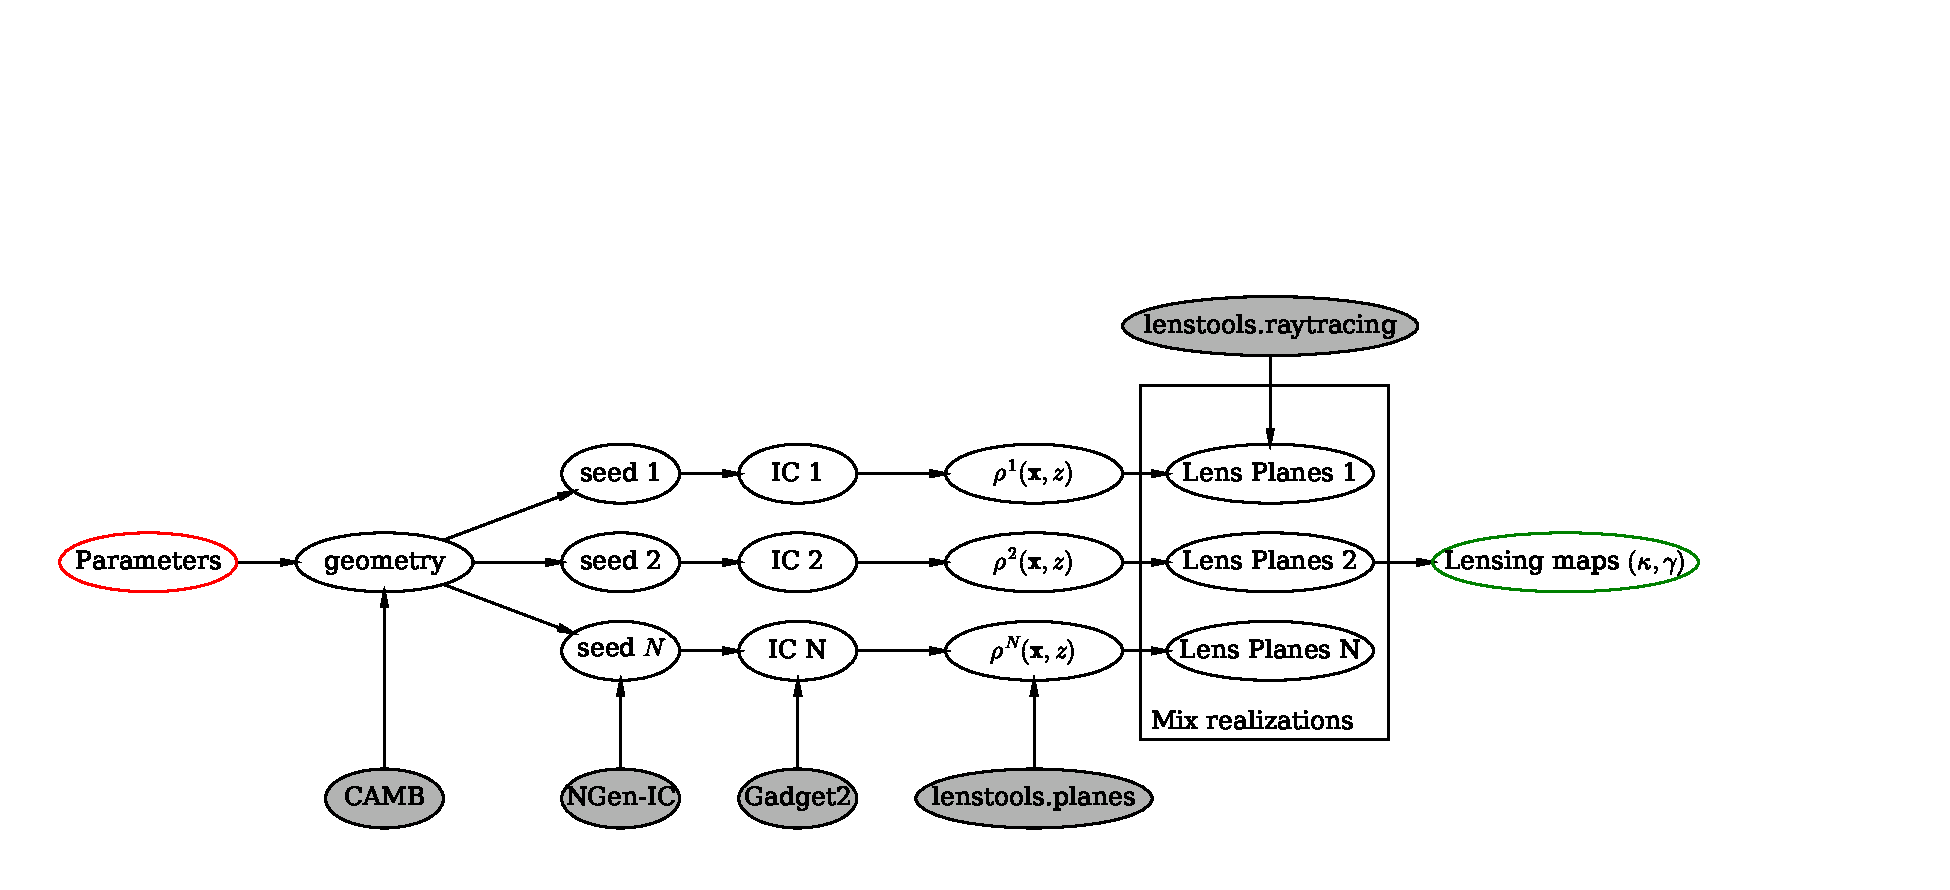
\includegraphics[scale=0.6]{Figures/flow.eps}
\caption{Workflow of the \LT WL shear simulation operations, from the specifications of the cosmological parameters $\bb{p}$ to the finished image products.}
\label{pipescheme}
\end{figure*}

\subsection{Pipeline code structure}
%
In this paragraph we describe how the \LT pipeline code is organized. The simulation products are placed in a directory tree structure which is optimized for easy resource access. The directory tree is mirrored in two locations, a so called \textit{Home} location, which holds all the book--keeping information such as configuration files and a \textit{Storage} location which holds the simulation products (\ttt{Gadget2} snapshots, lens planes and finished shear maps). The reason for this is that while the \textit{Home} location does not require much disk space, the \textit{Storage} location can reach disk sizes of several Terabytes. We found convenient to keep the two locations separated to ensure product management, sharing and portability between different computer clusters. The directory tree is organized as in Figure \ref{inheritance}. A batch of simulations is handled by a single instance of a \ttt{SimulationBatch} object (which holds both the \textit{Home} and \textit{Storage} parts). The first level in the tree corresponds to a specifications of cosmological parameters $\bb{p}$: each node on this level is an instance of the \ttt{SimulationModel} class. The second level in the tree specifies the size and resolution of the $N$--body box, namely the box size $L_b$ and the number of particles $N_p$: each node on the second level is an instance of the \ttt{SimulationCollection} class. Inside a simulation collection, we are free to choose different random realizations of the initial conditions, which will then be evolved in time by the $N$--body code. Each such realization lives on a node which is one level deeper in the tree, and is encoded in a \ttt{SimulationIC} object. The deepest level in the tree contains the two dimensional slices of the $N$--body simulation boxes. Each node on this level is an instance of the \ttt{SimulationPlanes} class. Once the lens planes are generated, the ray--tracing operations can be performed. In principle we can use lens planes that live under the same \ttt{SimulationCollection}, but belong to different \ttt{SimulationIC} nodes, to produce either single redshift shear images (each ensemble of images lives in a \ttt{SimulationMaps} object) or shear calalogs of $N_g$ sources, in the form of a table in which each of the $N_g$ rows is a tuple $(x_g,y_g,z_g,\gamma_{1,g},\gamma_{2,g})$. Each ensemble of catalogs corresponds to an instance of the \ttt{SimulationCatalog} class. Note that, because they combine different initial conditions, both \ttt{SimulationMaps} and \ttt{SimulationCatalog} nodes live on the same level of the directory tree, one level below \ttt{SimulationCollection}. An example on how to create a \ttt{python} script to lay down such a directory tree is shown in the Appendix A.     

\begin{figure*}
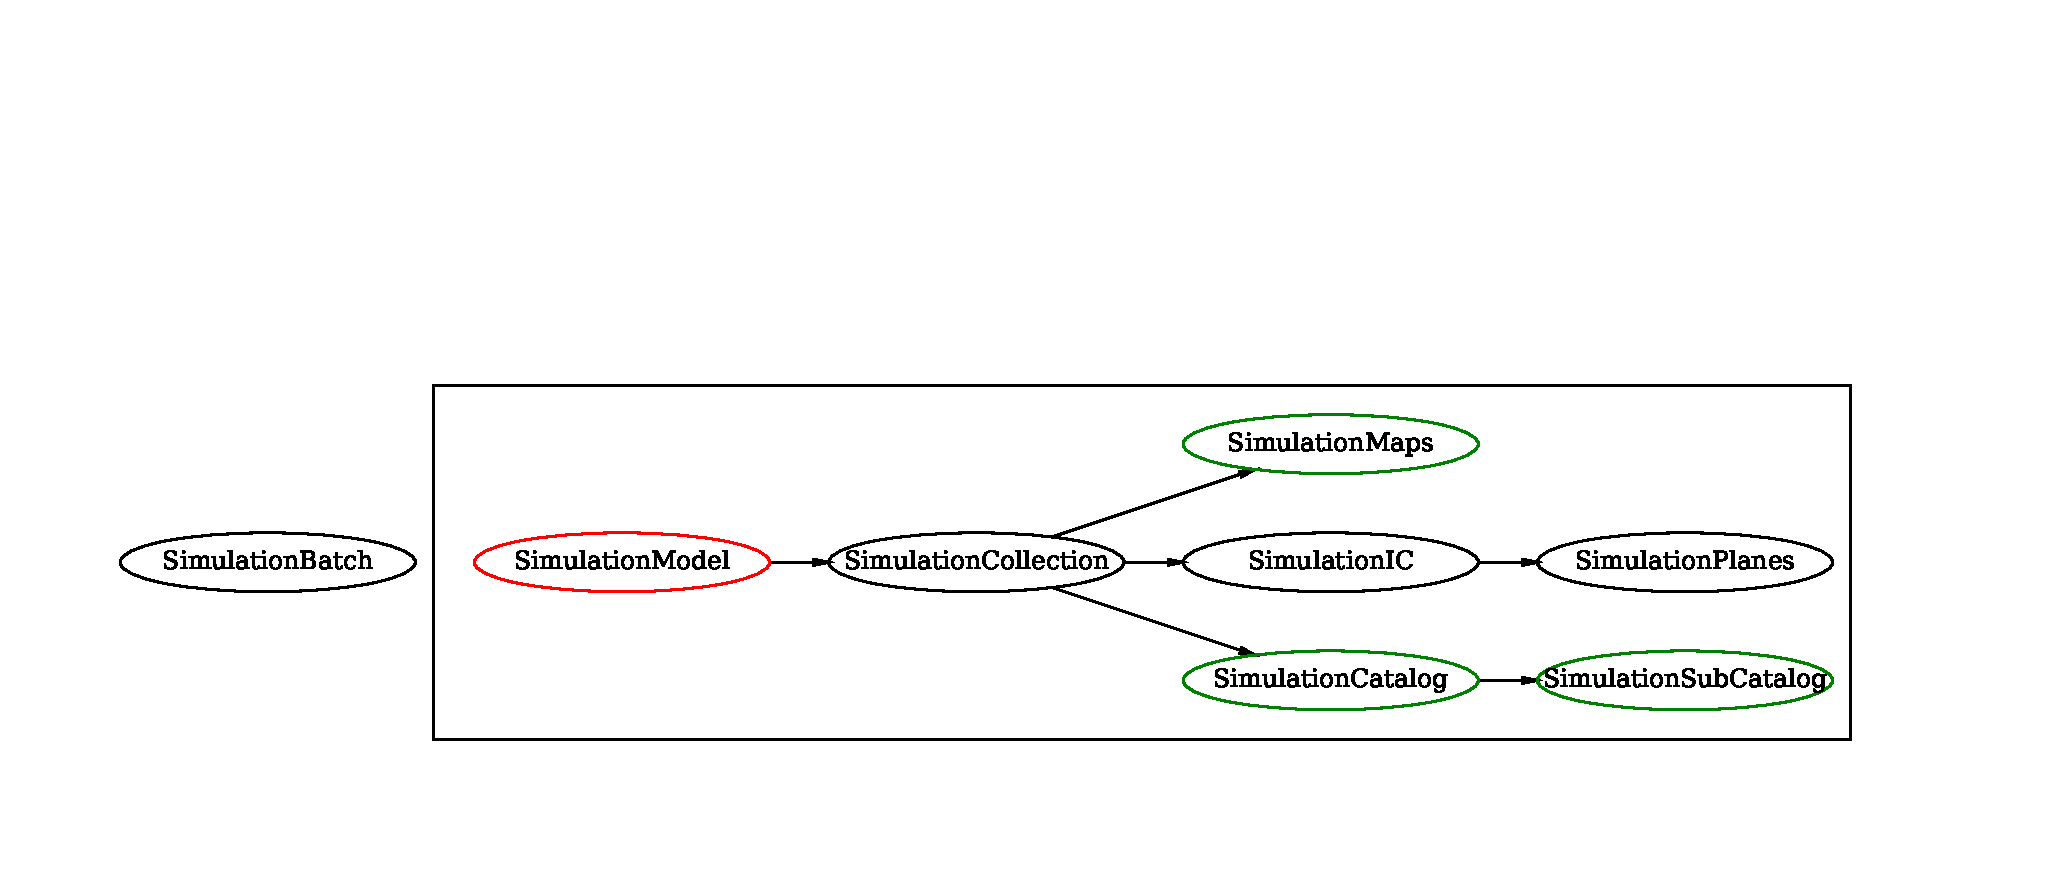
\includegraphics[scale=0.6]{Figures/inheritance.eps}
\caption{Directory tree structure and corresponding class inheritance in the \LT shear simulation operations.}
\label{inheritance}
\end{figure*}

\subsection{Performance}
%
We summarize the runtime and memory usage benchmarks of the \LT shear simulation pipeline. The tests were run on the TACC Stampede computer cluster\footnote{\url{https://portal.xsede.org/tacc-stampede}}. Table \ref{benchmarktable} shows a summary of the ray--tracing operations performed by \LT, indicating the complexity and runtime of each operation for a selected test case. At the lens plane generation stage we can clearly see that the two bottlenecks in the flow are the $N$--body snapshot read operations and the Poisson equation solving via FFT. We can optimize the number of tasks $N_t$ used to read in a single snapshot because, in the limit of perfect parallel input performance, there is an optimal value of $N_t(N_p,L_p)$ that minimizes the combined input, gridding and MPI communication operations, which have a combined complexity

\begin{equation}
t_{\rm in+grid+MPI} = A_1\frac{N_p}{N_t} + A_2L_p\log{N_t}
\end{equation} 
%
The optimal $N_t$ depends on the number of particles $N_p$ and the lens plane resolution (in pixels) $L_p$. The Poisson solving operations have a complexity of $O(L_p\log{L_p})$ which is dominated by the FFT performance. Although we make use of the \ttt{numpy} FFT pack \citep{scipy} to perform such operations, other alternatives are also possible (such as FFTW \citep{FFTW05}). The \LT code modularity makes it very easy to switch between different implementations of the FFT algorithm.  

We also tracked the memory usage of the lens plane and ray--tracing operations. This is an important step, since \ttt{python} has some subtleties when dealing with large memory applications. The total memory allocated by a \ttt{python} process never decreases, even if the resources are released (of course the freed memory can be re--used by newly allocated resources without increasing the peak memory of the \ttt{python} process). Figure \ref{memoryfig} shows the peak memory usage during the lens plane generation and ray--tracing operations. We can see that, for the test case outlined in Table \ref{benchmarktable}, memory consumption stabilizes around 1.3\,GB per task for the lens planes and 1.8\,GB per task during the ray--tracing. These considerations make the \LT pipeline suitable for deployment on computer clusters with $\gtrsim$2\,GB memory per core, such as the one we used.    

\begin{table*}
\begin{tabular}{l|c|c|c}
\toprule
{Step} &            Complexity &            Test case &           Runtime \\ \hline \hline
\midrule
\multicolumn{4}{c}{\textbf{Lens generation}} \\ \hline
Snapshot input & $O(N_p/N_t)$  & $N_p=512^3$, $N_t=16$  & 2.10\,s  \\
Gridding        & $O(N_p/N_t)$   & $N_p=512^3$, $N_t=16$  & 0.20\,s \\
MPI Communication  & $O(L_p\log{N_t})$   & $N_t=16$, $L_p=4096^2$  & 0.76\,s   \\
Poisson solver (FFT)           & $O(L_p\log{L_p})$ & $L_p=4096^2$  &  2.78\,s    \\
Lens output           & $O(L_p)$ & $L_p=4096^2$   & 0.04\,s  \\ \hline \hline

\multicolumn{4}{c}{\textbf{Ray tracing}} \\ \hline
Lens input &  $O(L_p)$ & $L_p=4096^2$ & 0.32\,s \\
Random lens shift &  $O(L_p)$ & $L_p=4096^2$ & 0.15\,s \\
Deflection calculation        &  $O(N_r)$ & $N_r=2048^2$   & 1.54\,s  \\
Shear tensor product               &  $O(N_r)$ & $N_r=2048^2$   &  1.29\,s \\ \hline \hline

\bottomrule
\end{tabular}
\caption{Summary of the ray--tracing benchmarks: each $N$--body snapshot is divided in $N_t$ files, which are read in parallel and contain a total of $N_p$ particles. After the gridding procedure (\ref{surfacedensity}) is performed by each task, the total sufrace density (computed for a plane of $L_p$ pixels) is collected by the master task, which then proceeds in solving the Poission equation (\ref{poisson}) via Fast Fourier Transforms and saves the output to disk. In a subsequent step, the lens densities are read from disk, and the geodesic equations (\ref{geodesic2D}) are solved for $N_r$ different starting positions $\pmb{\theta}$ that allow to reconstruct the shear and convergence fields $\pmb{\gamma},\kappa$.}
\label{benchmarktable}
\end{table*}

\begin{figure}
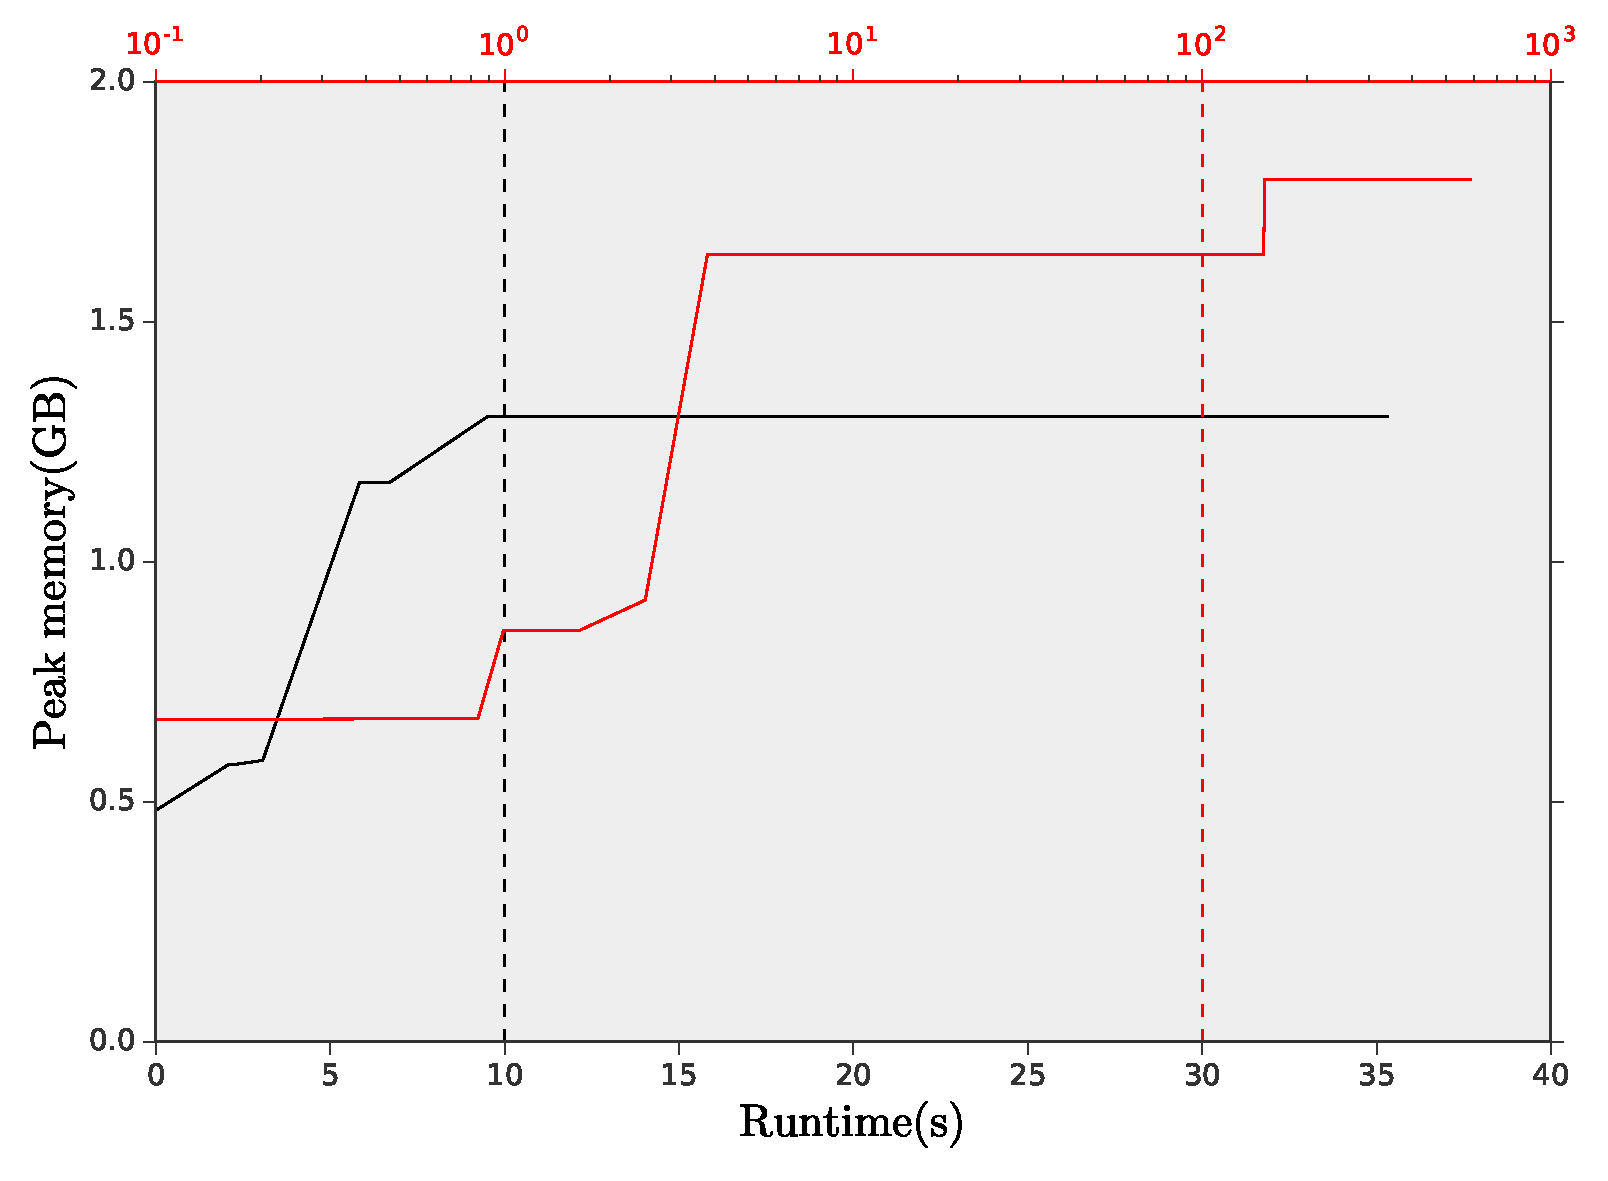
\includegraphics[scale=0.3]{Figures/memory_usage.eps}
\caption{Peak memory usage for the lens plane generation (black) and ray--tracing (red) as a function of runtime $t$ for the test case indicated in Table \ref{benchmarktable}. The vertical lines are drawn in correspondence of the completion of a lens plane calculation (black) and a lens crossing (red).}
\label{memoryfig}
\end{figure}

%%%%%%%%%%%%%%%%%%%%%%%%%%%%%%%%%%%%%%%%%%%%%%%%%%%%%%%%%%%%%%%%%%%%%%%%%%%%%%%%%%%%%%%%%%%%%%%%%%%%%%%%%%%%%%%%%%%%%%%%%%%%%%%%%%%%%%%%%%%%%

\section{Image analysis}
%

\begin{equation}
\langle\tilde{\kappa}(\pmb{\ell})\tilde{\kappa}(\pmb{\ell}^\prime)\rangle = (2\pi)^2\delta_D(\pmb{\ell}+\pmb{\ell}^\prime)P^{\kappa\kappa}(\ell)
\end{equation}
%
In term of the $E$ and $B$ modes defined as

\begin{equation}
\label{ebmodeeqs}
\begin{matrix}
E(\pmb{\ell}) = \frac{(\ell_x^2-\ell_y^2)\tilde{\gamma}^1(\pmb{\ell})+2\ell_x\ell_y\tilde{\gamma}^2(\pmb{\ell})}{\ell_x^2+\ell_y^2}  \\ \\
B(\pmb{\ell}) = \frac{-2\ell_x\ell_y\tilde{\gamma}^1(\pmb{\ell})+(\ell_x^2-\ell_y^2)\tilde{\gamma}^2(\pmb{\ell})}{\ell_x^2+\ell_y^2}
\end{matrix}
\end{equation}
%
we have $E=O(\phi)$ and $B=O(\phi^2)$. The $E$--mode is the convergence $\kappa$, hence $P^{EE}=P^{\kappa\kappa}$.  

\begin{figure*}
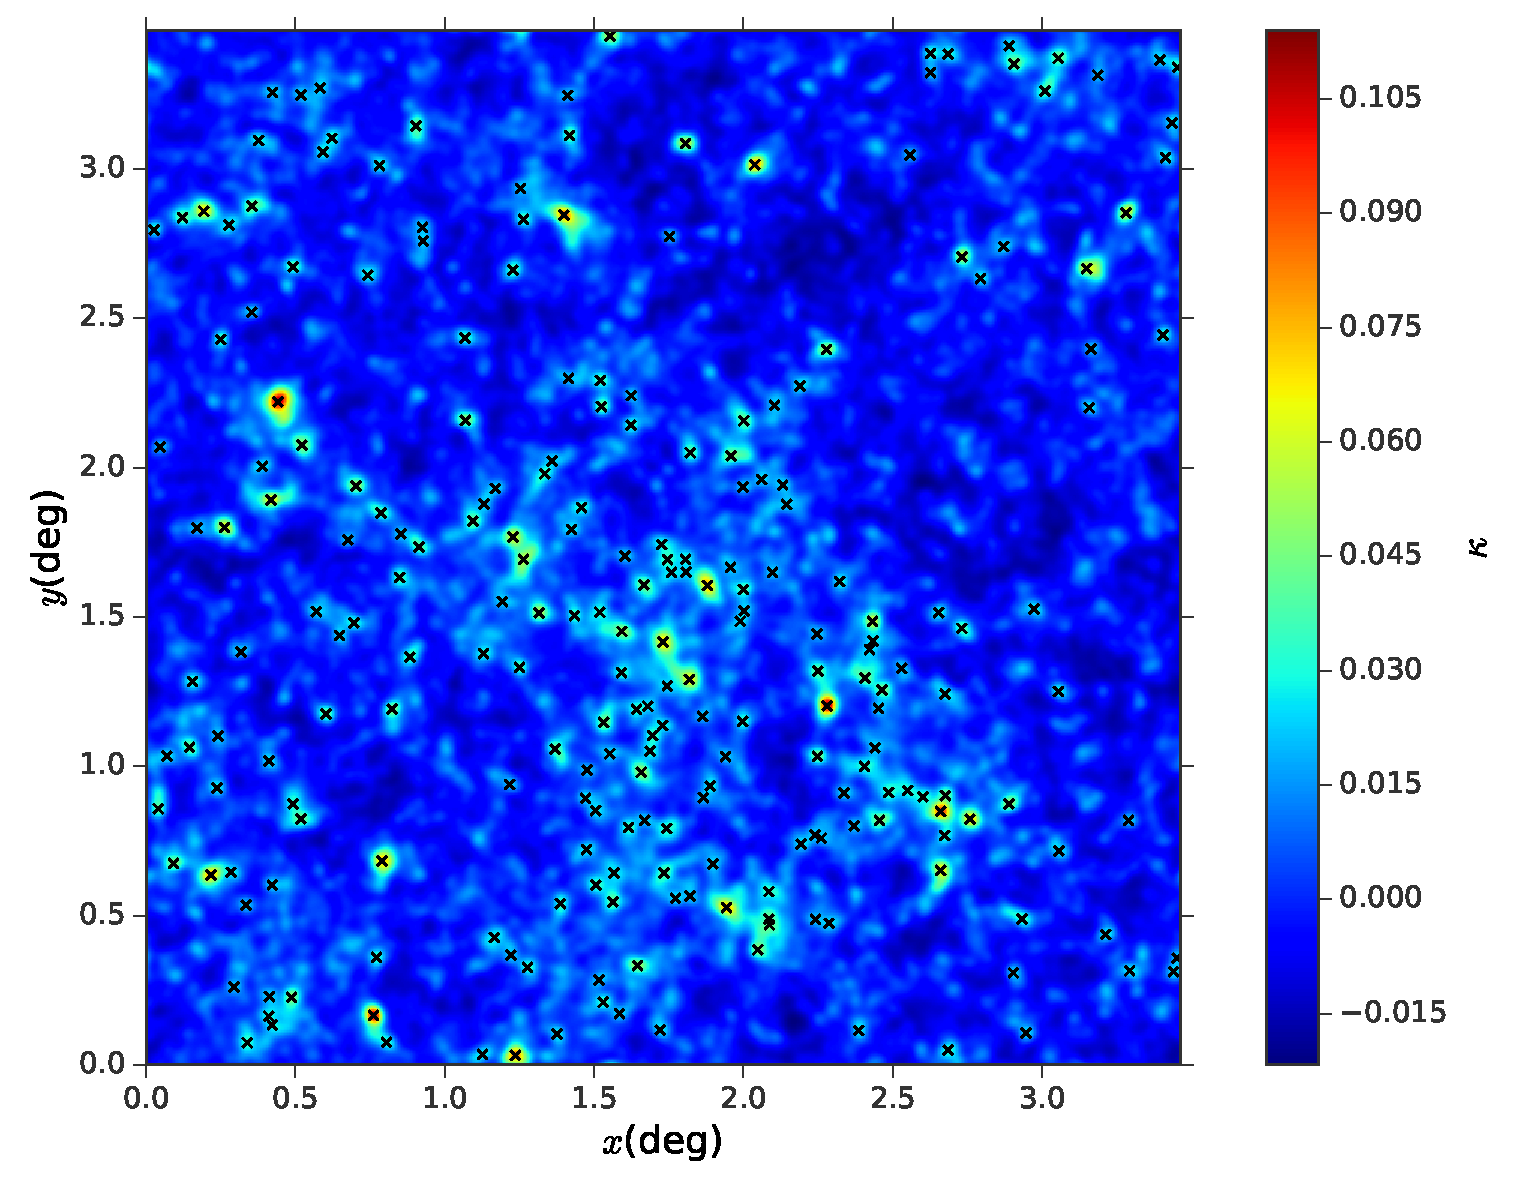
\includegraphics[scale=0.3]{Figures/convergence_visualize.eps}
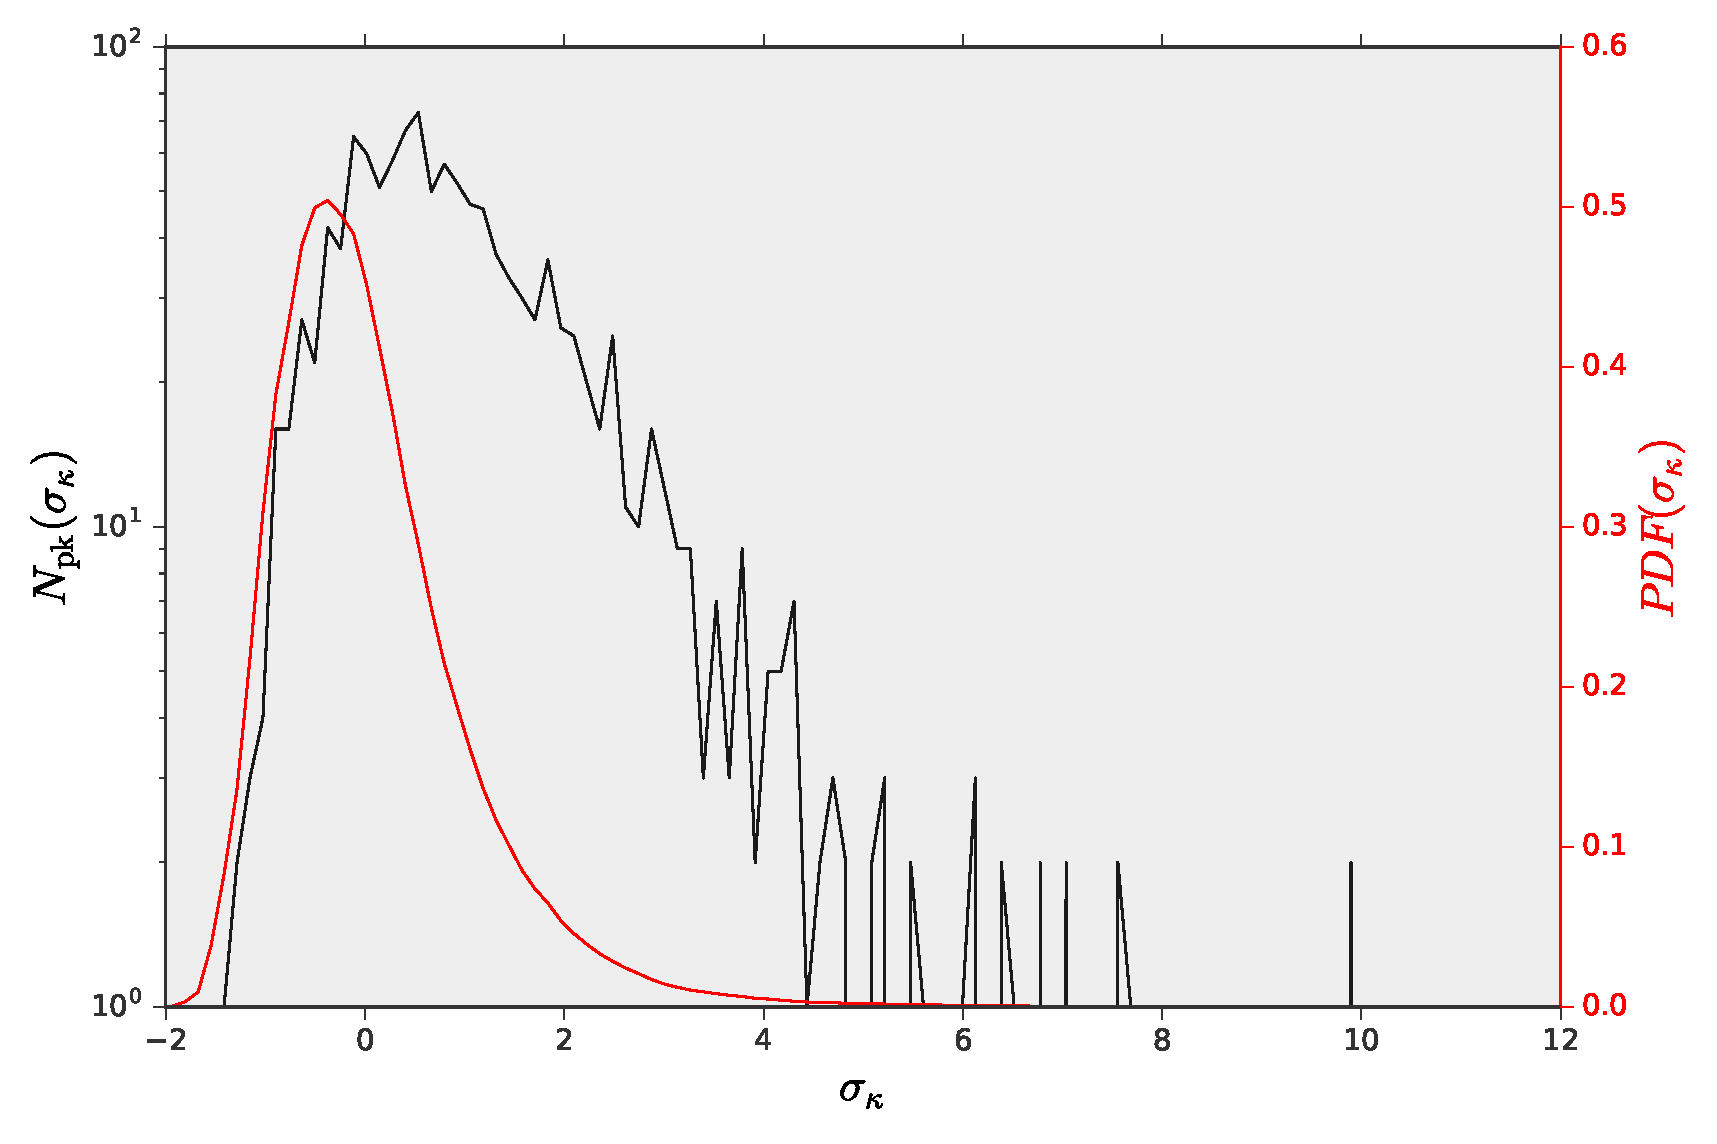
\includegraphics[scale=0.3]{Figures/convergence_stats.eps}
\caption{One of the convergence maps produced with the \LT shear simulation pipeline. The map has been generated assuming a uniform background source distribution at $z_s=2$ and has an angular size of $3.5^\circ$ and a resolution of 2048 pixels per side, which correspond to a pixel resolution of $0.1^\prime$. The black crosses in the left panel identify local maxima (\textit{peaks}) in the $\kappa$ field with a significance of at least 2$\sigma$. The right panel shows the PDF of the $\kappa$ field (red) and its peak histogram (black).}
\label{convergencefig}
\end{figure*}

\begin{figure}
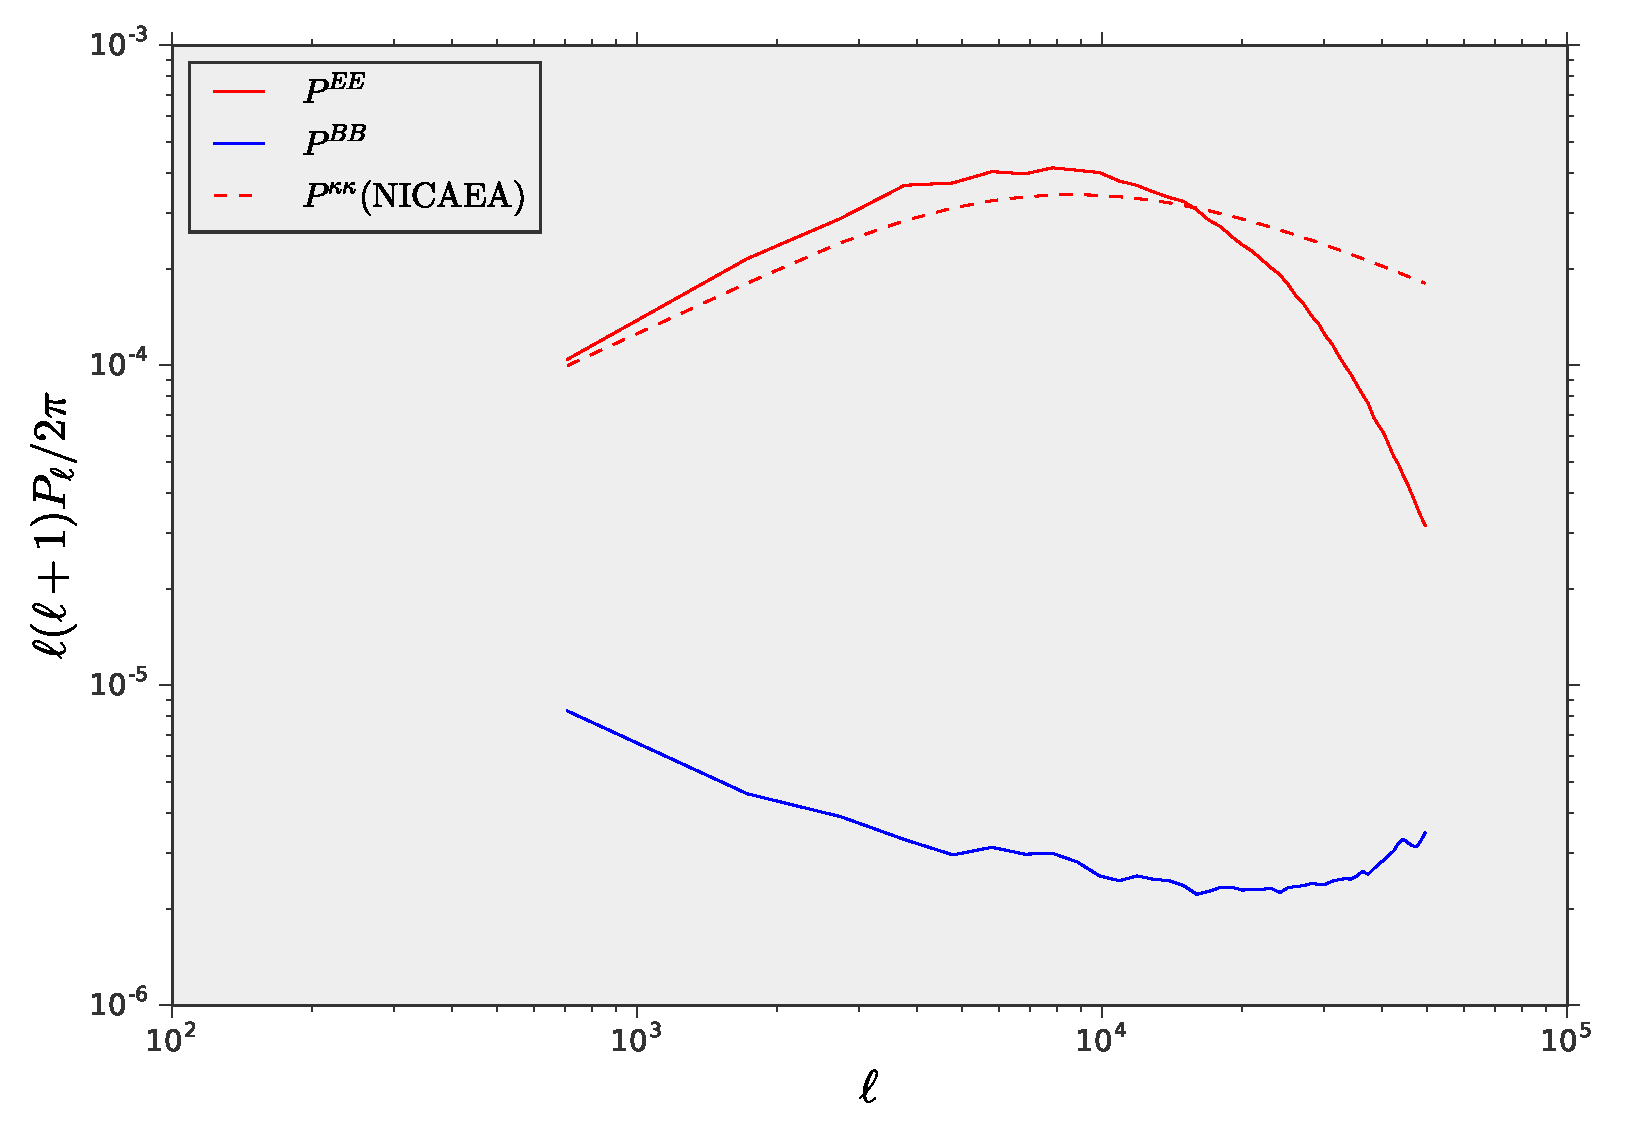
\includegraphics[scale=0.3]{Figures/eb_modes.eps}
\caption{$E$ and $B$ mode power spectra of one of the shear maps generated with the \LT simulation pipeline. We show the $E$--mode power spectrum $P^{EE}$ (red) and the $B$--mode power spectrum (blue), computed using equation (\ref{ebmodeeqs}) We also show an analytical prediction of the $\kappa$ power spectrum obtained with the public code \ttt{Nicaea} (dashed red line).}
\label{ebmodefig}
\end{figure}


%%%%%%%%%%%%%%%%%%%%%%%%%%%%%%%%%%%%%%%%%%%%%%%%%%%%%%%%%%%%%%%%%%%%%%%%%%%%%%%%%%%%%%%%%%%%%%%%%%%%%%%%%%%%%%%%%%%%%%%%%%%%%%%%%%%%%%%%%%%%%

\section{Cosmology constraints}

\begin{figure}
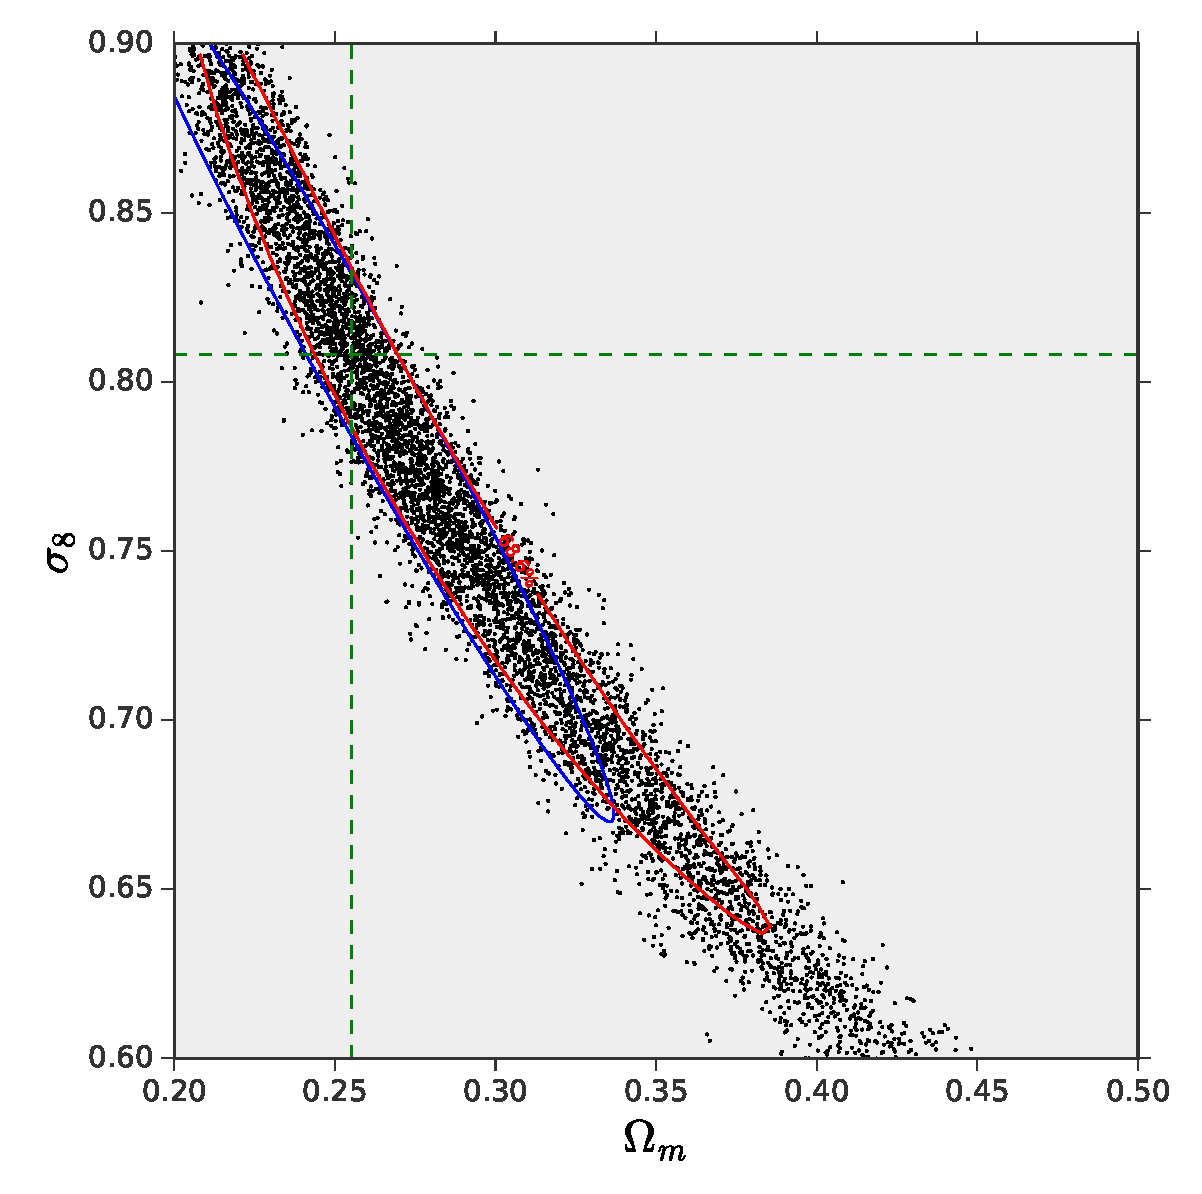
\includegraphics[scale=0.4]{Figures/parameter_sampling.eps}
\caption{Cosmological constraints based on the sampling of the parameter space $(\Omega_m,\sigma_8)$ with three different techniques. We use a grid evaluation of the likelihood function based on a Radial Basis Function emulator (red), a Fisher matrix calculation (blue) and a MCMC sampling using the \ttt{emcee} package (black dots). The covariance matrix $\bb{C}$ has been estimated from 1024 random realizations of the feature vector, produced with the \LT shear simulation pipeline.}
\label{samplingfig}
\end{figure}

%%%%%%%%%%%%%%%%%% FUTURE %%%%%%%%%%%%%%%%%%%%%%%%%%%%%%%%%%%%%

\section{Future developments}

%%%%%%%%%%%%%%%%%% CONCLUSION %%%%%%%%%%%%%%%%%%%%%%%%%%%%%%%%%%%%%

\section{Conclusion}

%%%%%%%%%%%%%%%%%%%%%%%%%% ACKNOWLEDGMENTS %%%%%%%%%%%%%%%%%%%%%%%%%%%%%%%%%%%%%%%%%%%%%%%%%%%%%%
 

\section*{Acknowledgements}

%%%%%%%%%%%%%%%%%%%%%%%%%% APPENDIX: CODE SNIPPETS %%%%%%%%%%%%%%%%%%%%%%%%%%%%%%%%%%%%%%%%%%%%%%%%%%%%%%

\section*{Appendix: code snippets}

\subsection{Pipeline directory tree}


\bibliography{ref}
\label{lastpage}
\end{document}
